\begin{remarkBox}{Some Properties of Inverse Image}
    Let \( f: X \rightarrow Y \) be a function. 
    Let \( \{ B_{ i } \}_{ i \in I } \) be an indexed set of subsets of the 
    codomain \( Y \).
    Then 
    \begin{equation*}
        f^{ -1 }
        \left(
            \bigcup _{ i \in I } B_{ i }
        \right)
        =
        \bigcup _{ i \in I } f^{ -1 } ( B_{ i } )
        \quad \mathrm{and} \quad 
        f^{ -1 }
        \left(
            \bigcap _{ i \in I } B_{ i }
        \right)
        =
        \bigcap _{ i \in I } f^{ -1 } ( B_{ i } )
    \end{equation*}
    It is as if the inverse image commutes with unions and intersections.
\end{remarkBox}

\begin{remarkBox}{Some Properties of Images}
    Let \( f: X \rightarrow Y \) be a function. 
    Let \( \{ A_{ i } \}_{ i \in I } \) be an indexed set of subsets of the 
    domain \( X \).
    Then 
    \begin{equation*}
        f
        \left(
            \bigcup_{ i \in I } A_{ i }
        \right)
        =
        \bigcup_{ i \in I } f ( A_{ i } )
    \end{equation*}
    Notice that the same cannot be said of intersections in this case -- 
    we can say 
    \begin{equation*}
        f
        \left(
            \bigcap_{ i \in I } A_{ i }
        \right)
        \subset
        \bigcap_{ i \in I } f ( A_{ i } )
    \end{equation*}

    \baseSkip

    Take for example \( f: \mathbb{R} \rightarrow \mathbb{R} \) with
    \( f ( x ) = x^{ 2 } \) as its formula. 
    Let \( A = ( - \infty, 0 ] \) and \( B = [ 0, \infty ) \).
    Then we see that 
    \begin{equation*}
        f ( A \cap B )
        =
        \{ 0 \}
        \quad \mathrm{but} \quad
        f ( A ) \cap f ( B ) = [ 0, \infty )
    \end{equation*}
\end{remarkBox}

\begin{remarkBox}{On Continuity}
    Continuity of a function depends not only upon the function \( f \) itself,
    but also on the topologies specified for its domain and range.
\end{remarkBox}

\begin{remarkBox}{Differences Between Definitions of Continuity}
    Notice that Munkres uses the definition of continuity that involves 
    inverse images.
    However, we introduced the definition of continuity that involves 
    images; the main reason being that this definition is more intuitive to
    understand.
    All the other definitions of continuity (say, in analysis) were framed 
    using images, so it seems natural that the topological definitions
    follows in those same footsteps.

    \baseSkip
    
    In analysis, a function \( f: \mathbb{R} \rightarrow \mathbb{R} \) is 
    said to be continuous at a particular point \( p \in \mathbb{R} \) if and
    only if 
    \begin{equation*}
        \forall \epsilon > 0, \exists \delta > 0 \text{ s.t. }
        \lvert f ( x ) - f ( p ) \rvert < \epsilon
        \text{ whenever } \lvert x - p \rvert < \delta
    \end{equation*}
    We can phrase this instead in terms of open balls. In \( \mathbb{R} \), an
    open ball of radius \( r \) centered at \( p \) is really jus the open 
    interval \( B_{ r }( p ) = ( p - r, p + r ) \).
    We can further rephrase this in terms of inequalities: a point \( x \)
    is in \( B_{ r }( p ) \) if and only if \( \lvert x - p \rvert < r \).

    \baseSkip 
    
    Using this change of phrase, we can give an alternative definition for
    continuity. We say that \( f: \mathbb{R} \rightarrow \mathbb{R} \) is
    continuous at \( p \) if and only if:
    \begin{equation*}
        \forall \epsilon > 0, \exists \delta > 0 \text{ s.t. }
        f ( x ) \in B_{ \epsilon }( f ( p ) ) 
        \text{ whenever } x \in B_{ \delta }( p )
    \end{equation*}
    This definition is more in line with the topological definition we had 
    for continuity.
    
    \baseSkip

    Although the definition of continuity involving images is more intuitive,
    it is not as useful as the definition of continuity involving inverse 
    images.
    This is because inverse images have much nicer properties than images, so
    it makes it easier to work with when solving problems.
\end{remarkBox}

\begin{remarkBox}{Why we need the inverse function to be continuous}
    The condition that \( f^{ -1 } \) is continuous says that for 
    each open set \( U \) of \( X \), the inverse image of \( U \) under the map
    \( f^{ -1 }: Y \rightarrow X \) is open in \( Y \).
    However, notice that the inverse image of \( U \) under the map 
    \( f^{ -1 } \) is the same as the image of \( U \) under the map \( f \). 

    \begin{figure}[H]
        \centering
        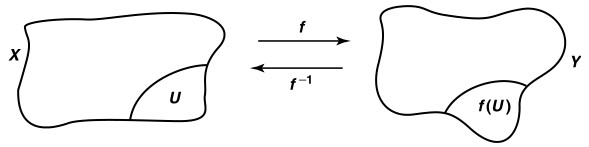
\includegraphics[ width = 0.6\linewidth ]{figures/Section 18/rem18-1.jpg}
        \caption{A visual for homeomorphisms}
        \label{fig:18-3}
    \end{figure}
\end{remarkBox}

\begin{remarkBox}{On Equivalent Definitions of Homeomorphisms}
    These equivalent definitions shows that a homeomorphism 
    \( f: X \rightarrow Y \) gives us a bijective correspondence not only
    between \( X \) and \( Y \), but also between the collection of open sets
    of \( X \) and of \( Y \).
\end{remarkBox}

\begin{remarkBox}{Analogy of Homeomorphism to Isomorphism}
    In algebra, we have studied the notion of an isomorphism between algebraic 
    objects such as groups or rings.
    An isomorphism is a bijective correspondence that preserves the algebraic
    structure involved.

    \baseSkip

    The analogous concept in topology is that of homeomorphism; it is a 
    bijective correspondence that preserves the topological structure involved.
\end{remarkBox}

\begin{remarkBox}{More Examples}
    More examples can be found on \S 18 of Munkres.
\end{remarkBox}